\begin{surferIntroPage}{Weltrekord-Fl�chen}
    Eine Fl�che hei�t \emph{nicht-singul�r} oder \emph{glatt}, wenn sie keine spitzen Stellen oder Selbstdurchdringungen (\emph{Singularit�ten} genannt) hat, z.B.\ eine Kugel oder ein Torus, siehe Abbildung. 
    Dies ist so gut wie immer der Fall, wenn wir die
    Fl�che zuf�llig w�hlen. 
    \begin{center}
      \vspace{-0.2cm}
      \begin{tabular}{@{}c@{}c@{}c@{\quad}c@{}c@{}c@{}c@{}}
        \begin{tabular}{@{}c@{}}
          glatt:
        \end{tabular}
        &
        \begin{tabular}{@{}c@{}}
          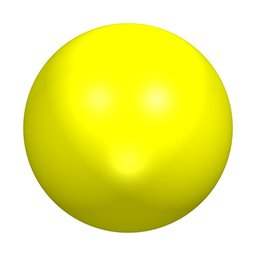
\includegraphics[width=1.1cm]{./../../common/images/kugel}
        \end{tabular}
        &
        \begin{tabular}{@{}c@{}}
          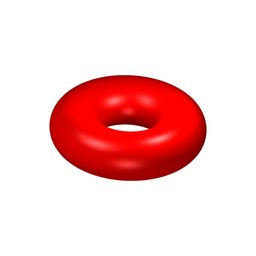
\includegraphics[width=1.1cm]{./../../common/images/torus}
        \end{tabular}
        &
        \begin{tabular}{@{}c@{}}
          viele\\
          Singularit�ten:
        \end{tabular}
        &
        \begin{tabular}{c@{}@{}}
          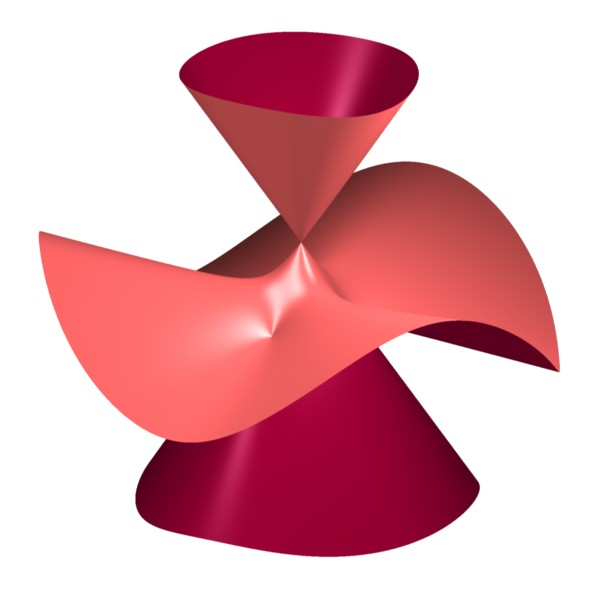
\includegraphics[width=1.1cm]{./../../common/images/cayley}
        \end{tabular}
        &
        \begin{tabular}{c@{}@{}}
          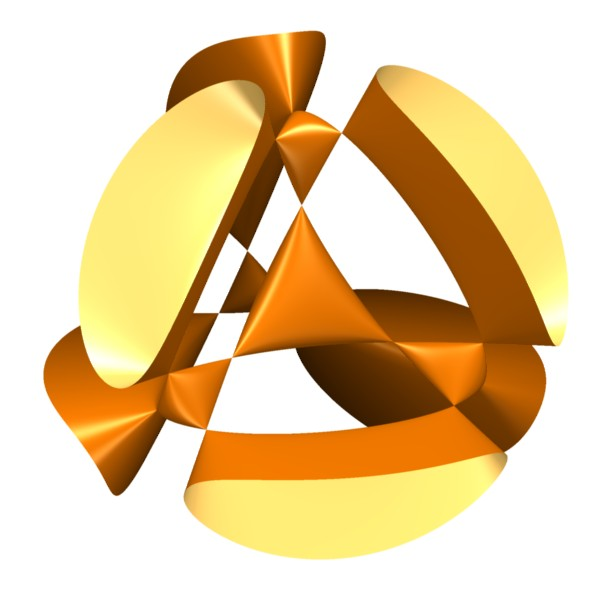
\includegraphics[width=1.1cm]{./../../common/images/kummer}
        \end{tabular}
        &
        \begin{tabular}{c@{}@{}}
          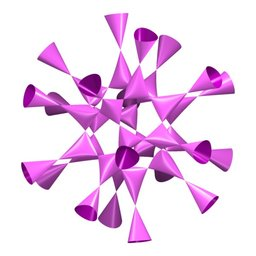
\includegraphics[width=1.1cm]{./../../common/images/barth_sextic}
        \end{tabular}
      \end{tabular}
    \end{center}
    \vspace{-0.2cm}
    Nur spezielle Fl�chen weisen Singularit�ten auf. Das macht diese Singularit�ten zu den interessantesten Punkten der Fl�che. 
    Alle Fl�chen im SURFER bestehen aus den Nullstellen von Polynomen. Das bedeutet, dass die Variablen in den Formeln nur ganzzahlige positive Exponenten haben. Den h�chsten Exponenten des Polynoms bezeichnet man auch als \emph{Grad} des Polynoms. 
    In der Mathematik lautet eine Frage in der Forschung wie viele Singularit�ten eine Fl�che mit einem bestimmten Grad haben kann. 
    Den Grad eines Polynoms bezeichnen wir mit $d$ und die Anzahl der Singularit�ten mit $\mu(d)$. Diese Zahl $\mu(d)$ ist sehr schwer zu ermitteln. F�r kleine Exponenten wie $d=1,2,3,4$ ist sie seit dem 19.\ Jahrhundert bekannt, doch f�r
    $d=5$ wurde die Zahl erst 1980 und f�r $d=6$ sogar erst 1996 herausgefunden.
    F�r ein Polynom vom Grad $7$ ist die maximale Anzahl der Singularit�ten bislang unbekannt. Es gibt jedoch schon einige Untersuchungen dazu.
    Eine endg�ltige Beantwortung der Frage f�r beliebiges $d$  liegt also noch in weiter Ferne.
    Einige bisher bekannte Werte:
    \begin{center}
      \begin{tabular}{r|cccccccc|c}
        $d$ & $1$ & $2$ & $3$ & $4$ & $5$ & $6$ & $7$ & $8$ & $d$\\
        \hline
        \hline
        \rule{0pt}{1.2em}$\mu(d)\ge$ & $0$ & $1$ & $4$ & $16$ & $31$ & $65$ &
        $99$ & $168$ & 
        $\approx \frac{5}{12}d^3$\\[0.3em]
        \hline
        \rule{0pt}{1.2em}$\mu(d)\le$ & $0$ & $1$ & $4$ & $16$ & $31$ & $65$ &
        $104$ & $174$ & $\approx \frac{4}{9}d^3$
      \end{tabular}
    \end{center}
\end{surferIntroPage}
